\documentclass[ams, a4j]{U-AizuGT}
\usepackage{pifont}
% \usepackage{graphicx}
\usepackage{cite}
\usepackage{mathtools}
% \usepackage{listings,jvlisting}
% \documentclass[a4j]{jarticle} %ここは関係ない
\usepackage{listings,jvlisting} 
\usepackage[dvipdfmx]{graphicx}
\usepackage{physics}

\usepackage[utf8]{inputenc}
\usepackage{booktabs} % きれいな表を作成するためのパッケージ

\bibliographystyle{ieicetr}

\lstset{
    frame=single,
    numbers=left,
    tabsize=2
}


% \usepackage{listings,jlisting}

% \lstset{%
%   language={C},
%   basicstyle={\small},%
%   identifierstyle={\small},%
%   commentstyle={\small\itshape},%
%   keywordstyle={\small\bfseries},%
%   ndkeywordstyle={\small},%
%   stringstyle={\small\ttfamily},
%   frame={tb},
%   breaklines=true,
%   columns=[l]{fullflexible},%
%   numbers=left,%
%   xrightmargin=0zw,%
%   xleftmargin=3zw,%
%   numberstyle={\scriptsize},%
%   stepnumber=1,
%   numbersep=1zw,%
%   lineskip=-0.5ex%
% }
\lstset{
  basicstyle={\ttfamily},
  identifierstyle={\small},
  commentstyle={\smallitshape},
  keywordstyle={\small\bfseries},
  ndkeywordstyle={\small},
  stringstyle={\small\ttfamily},
  frame={tb},
  breaklines=true,
  columns=[l]{fullflexible},
  numbers=left,
  xrightmargin=0zw,
  xleftmargin=3zw,
  numberstyle={\scriptsize},
  stepnumber=1,
  numbersep=1zw,
  lineskip=-0.5ex
}

% \bibliographystyle{ieice}
\author{Ryuki Hiwada}
\studentid{s1280076}
\supervisor{Naohito Nakasato}

\title{Domain Specific Language for high performance computing}

\begin{document}

\maketitle
\begin{abstract}

\end{abstract}
\section{Introduction}


\subsection{Background}

Particle simulations have been executed in various fields such as 
astrophysics and fluid dynamics. For example, N-body simulations 
simulate the dynamical evolution due to gravity between planets,
and models of fluid motion models simulate water.
Particle simulations are computationally demanding
with respect to the number of particles.
As an example, we will discuss the case of an N-body simulation.
In this simulation, most of the computational time is occupied by
the calculation of the gravitational interaction. equation \eqref{eq:gravity} is 
the equation for the gravitational interaction.

\begin{equation}
a_i = \sum_{\substack{j \neq i}}^{N} G m_j \frac{\vb{x}_j - \vb{x}_i}{\left( \left| \vb{x}_j - \vb{x}_i \right| + \epsilon^2 \right)^{3/2}\label{eq:gravity}}
\end{equation}

$a_i$, $\vb{x}_i$ $m_j$,$\vb{x}_j$,$N$,$G$,$\epsilon$
are the acceleration and position of particle i, the mass of particle j, the number of position particles, respectively, and
softening parameters to prevent gravitational constant divergence.
From equation \eqref{eq:gravity},time complexity is proportional to 
the number of particles N, 

 N-body simulations often require large numbers of particles.
For example, a globular cluster contains about $10^4 ~ 10^5 $ stars.
Therefore, very long computation time is required.  parallel computing is 
generally used to speed up the process.


The computation of interparticle interactions has high
data parallelism because the computation of particles is 
independent of each other. Therefore, 
Parallelism by SIMD\lparen Single Instruction/Multiple Data \rparen, 
one of Flynn's taxonomy \cite{flynn1972some} , is suitable.
SIMD means processing multiple data for a single instruction.
However, to perform SIMD, code must be written for the computer architecture.

The goal of this study is to allow users to run particle interaction 
calculations in parallel without having to be aware of parallelization.
We developed a Domain Specific Language\lparen DSL \rparen called Pyker.
DSL is a programming language for solving specific problems.
Pyker generates parallelized code with SIMD instructions for the 
calculation of interactions from the definition of variables and 
the description of formulas.
The evaluation method for Pyker is to compare the performance of 
the automatic SIMD  performed by the C compiler with that of the 
SIMD by Pyker. 
For this purpose, we measured the execution time of the code that
does not adapt the SIMD instructions generated by Pyker for each 
of the three interaction calculations.
The execution time of the code that does not adapt SIMD instructions
generated from Pyker and the code that does adapt SIMD instructions 
are measured and compared.

In this paper, section 2 explains how Pyker defines the interparticle 
interaction equation, section 3 describes the process of code generation 
by Pyker, and section 4 presents the results of the performance evaluation
experiments.

\section{Definition of the interparticle interaction in Pyker}

\subsection{interparticle interaction}
we explain the needed for information to the calculate interparticle 
interaction with reference to the actual code.
gravity.cpp is the C++ source code that performs the calculation 
in equation \eqref{eq:gravity}.
\begin{lstlisting}[frame=single, caption=skeleton code, label=fuga]
                  
  for (int i = 0; i < n; i++) {
    double ax = 0.0;
    double ay = 0.0;
    double az = 0.0;

    for (int j = 0; j < n; j++) {
        double dx = double(xj[j][0] - xi[i][0]);
        double dy = double(xj[j][1] - xi[i][1]);
        double dz = double(xj[j][2] - xi[i][2]);
        double r2 = dx * dx + dy * dy + dz * dz + eps2;
        double ri2 = 1.0f / sqrt(r2); 
        
        double mr = mj[j] * ri2 * ri2 * ri2;

        ax += double(mr * dx);
        ay += double(mr * dy);
        az += double(mr * dz);
    }

    acci[i][0] = ax;
    acci[i][1] = ay;
    acci[i][2] = az;
}
\end{lstlisting}

We will explain how this code corresponds to the expression 
\eqref{eq:gravity}.
acci,xi,mj,xj,eps2 correspond to
 $a_i$, $\vb{x}_i$ $m_j$,$\vb{x}_j$,$N$,$\epsilon$ respectively.
The $G$ is not in the code because it can be calculated after the 
calculation of the interparticle interactions.


 From this code, we can see that the variables to store the results, 
the variables for particle i and particle j respectively, and the 
variables for $N$ and $G$ can be calculated after the calculation of 
the particle-particle interaction. The other variables have different 
processing and data structures.


 Therefore, there are three categories of information in a variable.
\begin{itemize}
  \item Whether the variable is a particle i, a particle j, a
  variable that stores the result, or any other variable
  \item The type information of the variable.
  \item Whether the variable is a vector or not
\end{itemize}

 With the definition of this variable and a description of the
mathematical equation using the variable, a code to calculate the
interparticle interaction can be generated.
これらをもとにPykerの言語仕様を説明する。

\subsection{language specification}
Pykerでは、大きく、変数定義と相互作用記述に分かれる。
まず変数定義について説明する。


 先ほどのセクションよりPykerの変数定義を以下に正規表現で示す。
% \begin{lstlisting}  
\["(EPI|EPJ|FORCE)?\:\text{ } (vec3<)?(F64)>?\:\text{ } \text{\textbackslash w+}"\]
% \end{lstlisting}
EPI,EPJ,FORCEはそれぞれ粒子i,粒子j,結果を保存する変数であることを示す。それ以外の変数は何も書かない
ベクトルはvec3で表す。
もしベクトルであれば'<>'の中に型を定義する。
型は倍精度小数だけでF64で示す。
最後に変数名を記述する。


次に相互作用記述の説明をする。
相互作用の記述に使える演算は以下の図に示す。

以下に\label{eq:gravity}の計算をPyker記述した例を示す。
\begin{lstlisting}[frame=single, caption=gravity\_interparticle, label=fuga]
  EPI vec3<F64> ri
  EPJ vec3<F64> rj
  EPJ F64 mass
  EPJ F64 eps2
  FORCE vec3<F64> ai
  rij = ri - rj
  r2 = rij * rij + eps2
  r_inv = 1.0 / sqrt(r2)
  r2_inv = r_inv * r_inv
  mr_inv = mass * r_inv
  mr3_inv = r2_inv * mr_inv
  ai = mr3_inv * rij
\end{lstlisting}

5行目までは変数定義部になる。



\begin{table}[ht]
  \centering % 表を中央揃えにする
  \caption{サンプル表} % 表のタイトル
  \label{tab:sampleTable}
  \begin{tabular}{ccc} % ここで列の数とテキストの配置を指定
  \toprule
  項目 & 値 & 単位 \\
  \midrule
  項目1 & 100 & kg \\
  項目2 & 200 & g \\
  項目3 & 300 & mg \\
\bottomrule
\end{tabular}
\end{table}



\section{Construction}
Pykerでは、どういうことができるのか?


We use Sympy, a library in Python for implementing  the implementation of pyker.
SymPy supports various operations, and the formulas using these operations are internally treated as 
syntax trees. We leveraged this functionality to read formulas and generate code capable of parallel execution.
For parallelization, we used an instruction set named Advanced Vector Extensions 2 \lparen AVX2\rparen. AVX2 is one of the 
extended instruction sets implemented in Intel's CPUs. The next section will explain how parallelization is carried out using AVX2.



\subsection{Pyker}
In this DSL, code is generated by writing and compiling two definitions: the definition of variables and the definition of interaction formulas. First, let us explain the variable definition.


In this DSL, variables are classified into classes: EPI, EPJ, FORCE, and others. EPI represents particles that receive interactions, 
while EPJ represents particles that provide interactions. FORCE holds the results of the interaction calculations, and other variables 
include softening parameters and the like. To perform calculations using these variables, in C++, it would be similar to \ref{fuga}.



\begin{lstlisting}[frame=single, caption=skeleton code, label=fuga]
int kernel(double xi[][3], double xj[][3], double ai[][3], double eps2, int n){
	// (1).preprocess
	for(int i = 0;i < n;i += 4) { // (2)Increment the number of parallels
		// (3).load EPI
		// (4).Initialization of tmporary force
		for(int j = 0;j < n;j += 1) {
        // (5) load EPJ
				// (6) calculate interparticle interactions
		}
		// (7). Store calculation result in the FORCE
	}
}
\end{lstlisting}

(1) involves preparatory steps such as defining variables necessary for the calculation. (2) 
involves loading the variables of EPI. (3) is about initializing variables that temporarily
 hold the results of the interaction calculation. (4) involves performing the interaction 
 calculation and saving the results in the primary variable of force. (5) involves storing the results in the FORCE variables.
To generate this code, in variable definition, information about the class of the variable,
 its type, and its dimension is necessary. Therefore, in pyker, variable definitions are written as follows. .
The first column, if it is a class, writes the name of the class and its member variable
 name. The second column explicitly writes the dimensions of the vector if there are any, 
 specifying 3 or 4 dimensions, and the type is either 32-bit or 64-bit floating-point. The 
 third column becomes the name of the variable handled on pykg. For example, "EPI.pos vec3<F64> xi" 
 would be a member variable of EPI named pos, a 3-dimensional 64-bit floating-point variable named xi.
The definition of interaction formulas is written to accumulate the results in the FORCE variable using
 the defined variables. Primary variables necessary for the mathematical description can be newly defined 
 using previously defined variables. Available operations include basic arithmetic, sqrt, and the power 
 symbol "**". The result is stored in the FORCE variable using '='.For instance, to generate code that c
 alculates the gravitational interaction formula shown in Figure 1, it would be written in this DSL as figure1.pyker.


\begin{lstlisting}[frame=single, caption=hoge, label=fuga]
EPI.pos vec3<F64> xi
EPJ.pos vec3<F64> xj
EPJ.m F64 mass
FORCE.acc vec3<F64> ai
F64 eps2
F64 g
dr = xj - xi
ai = g * mass *  dr / sqrt(dr ** 2 + eps2) ** 3
\end{lstlisting}
\subsection{Implementation}
The process of generating code is illustrated in the following flowchart. In Parsing, the information
of the variables defined in the DSL code is converted into a hash with the variable names as keys. 
Formulas are converted into syntax trees using the sympify() method of Sympy, and a list of these 
trees is obtained. Next, Common Subexpression Elimination (CSE) is performed on the syntax trees of the converted formulas. CSE is the process 
of reducing the number of operations by pre-calculating common subexpressions in formulas and using 
their results in subsequent calculations. In type inference, the types of the primary variables in the 
formulas are inferred. Afterward, all syntax trees are converted into binary trees to align them with 
SIMD operations. Finally, the code for calculating interactions is generated by traversing the processed 
syntax trees. The following sections describe how the implementation was carried out in the order of
Parsing, CSE, type inference, conversion to binary trees, and Code generation.
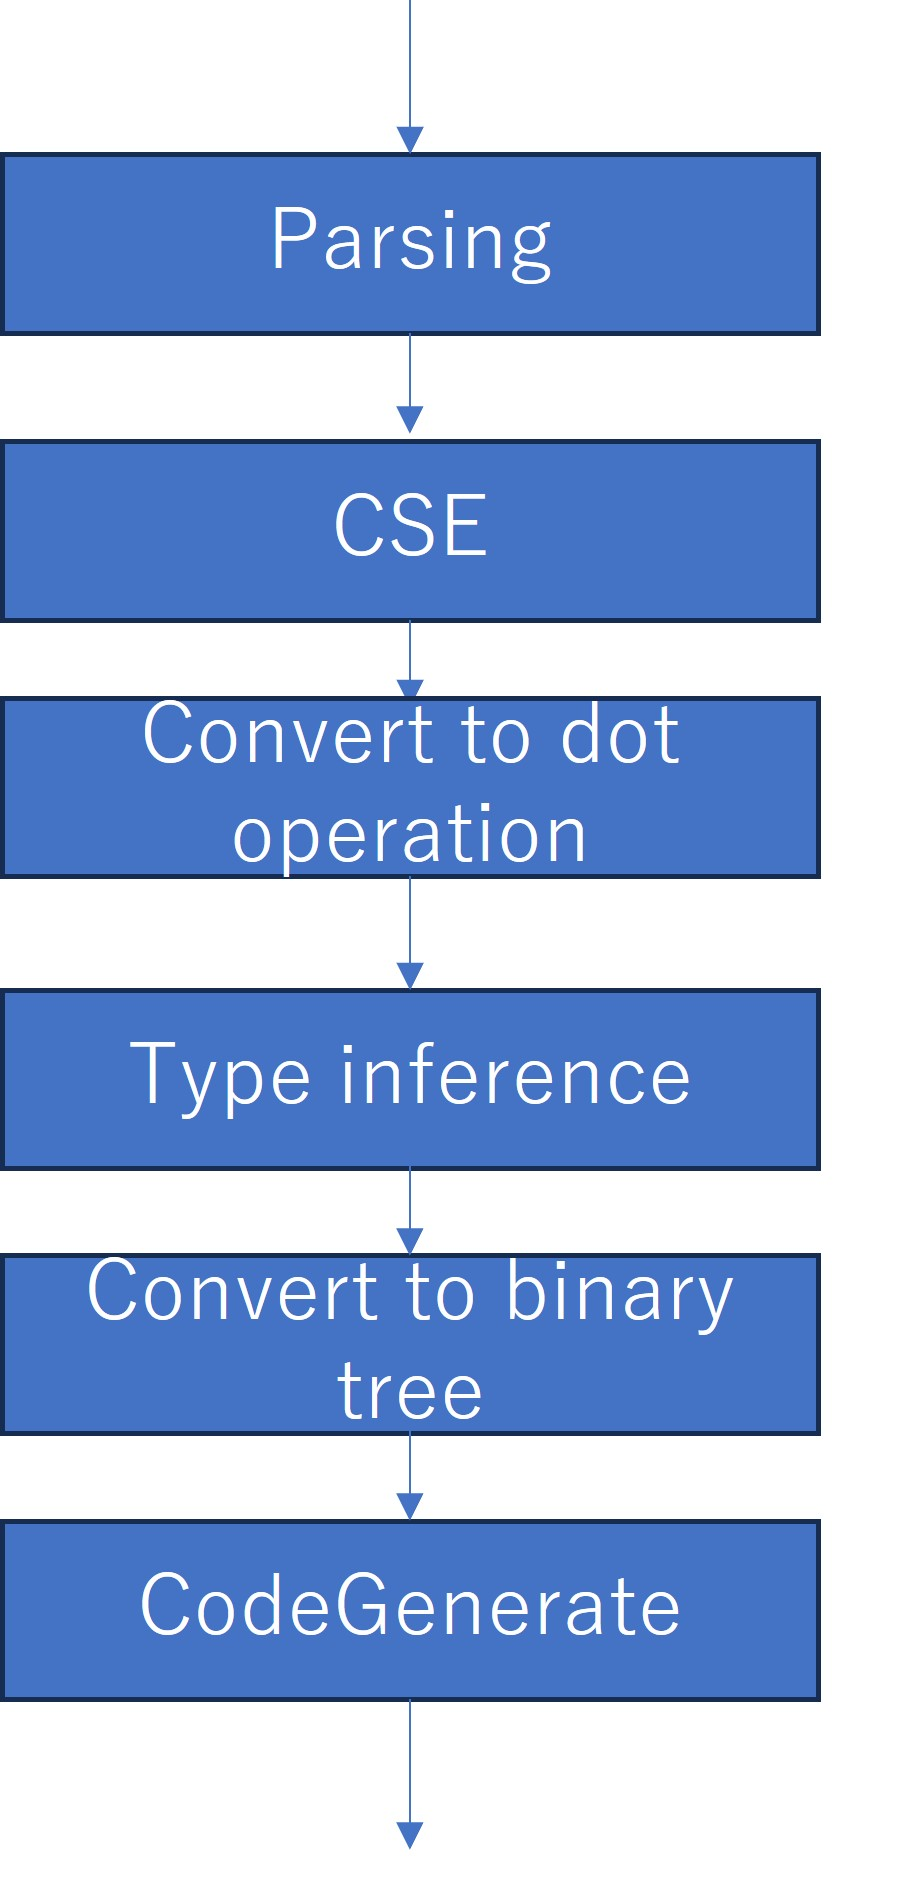
\includegraphics[width=0.2\textwidth]{flowchartver3.jpg}
\subsubsection{Parsing}
In Parsing, the process is divided between variable definition and formula handling. In variable definition, 
objects with class, vector, type, and variable name are created respectively. A hash with the variable name
as the key is then made (name\_variable\_map). Formulas use the sympify() method from the Sympy library to convert
the code read as a string into a syntax tree of formulas, obtaining a list of these syntax trees (expr\_list). Next, 
Common Subexpression Elimination (CSE) is performed.
\subsubsection{CSE}

\subsubsection{type inference}
\subsubsection{convert to binary trees}

\subsubsection{code generatation of non SIMD}


\subsubsection{code generatation of SIMD}




  
\section{Experiments}

\subsection{gravity interparticle}
ほぼ同じコードで実行


\begin{lstlisting}[frame=single, caption=Nbody-kernel.pyker, label=Nbody-kernel.pyker]
  EPI vec3<F64> ri
  EPJ vec3<F64> rj
  EPJ F64 mass
  EPJ F64 eps2
  FORCE vec3<F64> ai
  rij = ri - rj
  r2 = rij * rij + eps2
  r_inv = 1.0 / sqrt(r2)
  r2_inv = r_inv * r_inv
  mr_inv = mass * r_inv
  mr3_inv = r2_inv * mr_inv
  ai = mr3_inv * rij
  \end{lstlisting}

\begin{lstlisting}[frame=single, caption=Nbody-kernel.pikg, label=Nbody-kernel.pikg]
  EPI F64vec ri:r
  EPJ F64vec rj:r
  EPJ F64 mj:m
  EPJ F64 eps2:eps
  FORCE F64vec ai:acc
  rij = ri - rj
  r2 = rij * rij + eps2
  r_inv  = rsqrt(r2)
  r2_inv = r_inv * r_inv
  mr_inv  = mj * r_inv
  mr3_inv = r2_inv * mr_inv
  ai += mr3_inv * rij
  
\end{lstlisting}




non-simd

g++ -O3 

\begin{tabular}{|l|r|r|} \hline
  N & Pyker & PIKG \\ \hline
  25000 & 6.725156 & 4.444766 \\
  10000 & 0.738918sec & 0.517324sec \\


 \\ \hline
\end{tabular}


\begin{lstlisting}[frame=single, caption=Nbody-kernel.pikg, label=Nbody-kernel.pikg]
  g++ -O3 -I ~/school/PIKG/PIKG/inc -mavx2 -mfma gravity_interparticle.cpp
  
  \end{lstlisting}



  \begin{tabular}{|l|r|r|} \hline
    N & Pyker(sec) & PIKG(sec) \\ \hline
    50000 & 5.119071 & 3.333270\\
    25000 & 1.218129 & 1.148511 \\
    10000 & 0.143777 & 0.101594 \\
    1000 &  0.003521 & 0.002168 \\ \hline
  \end{tabular}
  
% \begin{tabular}{lrr}
%   N & pyker & PIKG \\
%   10000 & 0.143777sec & 0.101594sec \\
%   x & y & z 
%  \end{tabular}

\subsection{LennardJones}

\begin{lstlisting}[frame=single, caption=LennardJones-kernel.pyker, label=LennardJones-kernel.pyker]
EPI F64 rix
EPI F64 riy
EPI F64 riz
EPJ F64 rjx
EPJ F64 rjy
EPJ F64 rjz
EPJ F64 eps

FORCE F64 fx
FORCE F64 fy
FORCE F64 fz
FORCE F64 p
dx = rix - rjx
dy = riy - rjy
dz = riz - rjz
r2 = dx * dx + dy * dy + dz * dz + eps
r2i = 1.0 / r2
r6i = r2i * r2i * r2i
f = (48.0* r6i - 24.0) * r6i * r2i
fx = f * dx
fy = f * dy
fz = f * dz
p = 4.0 * (r6i) * (r6i - 1.0)
\end{lstlisting}
\begin{lstlisting}[frame=single, caption=LennardJones-kernel.pyker, label=LennardJones-kernel.pyker]
  EPI F64 rix:rx
  EPI F64 riy:ry
  EPI F64 riz:rz
  
  EPJ F64 rjx:rx
  EPJ F64 rjy:ry
  EPJ F64 rjz:rz
  EPJ F64 eps2:eps
  
  FORCE F64 fx:fx
  FORCE F64 fy:fy
  FORCE F64 fz:fz
  FORCE F64 p:p
  
  dx  = rix - rjx
  dy = riy - rjy
  dz  = riz - rjz
  r2  = dx * dx + dy * dy + dz * dz + eps2
  r2i = 1.0 / r2
  r6i = r2i * r2i * r2i
  f = (48.0 * r6i - 24.0) * r6i * r2i
  fx += f * dx
  fy += f * dy
  fz += f * dz
  p += 4.0 * r6i*(r6i - 1.0)

\end{lstlisting}


non-simd
\begin{tabular}{|l|r|r|} \hline
  N & Pyker & PIKG \\ \hline
  50000 & 40.736862 & 11.656278 \\
  25000 & 10.662050 & 3.521253 \\
  10000 & 0.985475 & 0.442775 \\
 \\ \hline
\end{tabular}


simd
\begin{tabular}{|l|r|r|} \hline
  N & Pyker & PIKG \\ \hline
  50000 & 3.702871  & 2.838773\\
  25000 & 0.838122 & 0.9904373 \\
  10000 & 0.134388 & 0.215270 \\

 \\ \hline
\end{tabular}



\section{Conclusion}
\section{Acknowledgement}

\begin{thebibliography}{99}
\end{thebibliography}
\bibliography{biblist}

\begin{table}[ht]
  \centering % 表を中央揃えにする
  \caption{サンプル表} % 表のタイトル
  \label{tab:sampleTable}
  \begin{tabular}{ccc} % ここで列の数とテキストの配置を指定
  \toprule
  項目 & 値 & 単位 \\
  \midrule
  項目1 & 100 & kg \\
  項目2 & 200 & g \\
  項目3 & 300 & mg \\
\bottomrule
\end{tabular}
\end{table}


\end{document}